\chapter{High Doping Concentrations in Nanowires}
\label{sec:high}

High ion fluences are needed to achieve high doping concentrations in a given structure. The simulations and experiments presented in this chapter where all performed with $175\, keV\,Mn^+$ irradiated $ZnO$ nanowires with approximately $200\,nm$ diameter; however, the conclusions also apply to other material combinations and structures. Some of the results presented in this chapter are also published in reference \cite{johannes_enhanced_2014}.

\section{Doping and Sputtering}

With \emph{iradina} the distribution of the places where the ions come to rest gives the profile of the concentration of dopants per ion fluence. Locally the concentration [$\nicefrac{atoms}{cm^{3}}$] increases a certain amount per fluence [$\nicefrac{ions}{cm^{2}}$], leading to the somewhat awkward unit of for the doping efficacy $[\nicefrac{(atoms/cm^{3})}{(ions/cm^{2})}]$. An example of the dopant distribution simulated with \emph{iradina} is shown in Figure \ref{iradinacrossection}a for the irradiation of a $200\,nm\,ZnO$ nanowire with $175\,keV\,Mn^+$. The ions enter the $y$-$z$ plane at random locations and at an angle of $45^\circ$ to the $z$-axis, which is periodically continued outside the plane of the image. It is clear that a homogeneous doping profile is not easy to obtain for the irradiation of a nanowire from one side. As with the creation of a box profile in bulk irradiations, multiple irradiation steps with varying energies are required. Note that an ion energy of $175\,keV$ is obviously not enough to permeate the whole nanowire diameter of $200\,nm$, so that an additional irradiation with higher ion energy would be required to obtain homogeneous doping. Rotating the nanowire under the ion beam is a much easier way of increasing the homogeneity of the doping profile. Figure \ref{iradinacrossection}b shows the local dopant incorporation efficacy for the rotation of the profile shown in \ref{iradinacrossection}a. Irradiation with a single, relatively low ion energy produces a homogeneous doping profile. 
  
\begin{Figure}
	\centering
		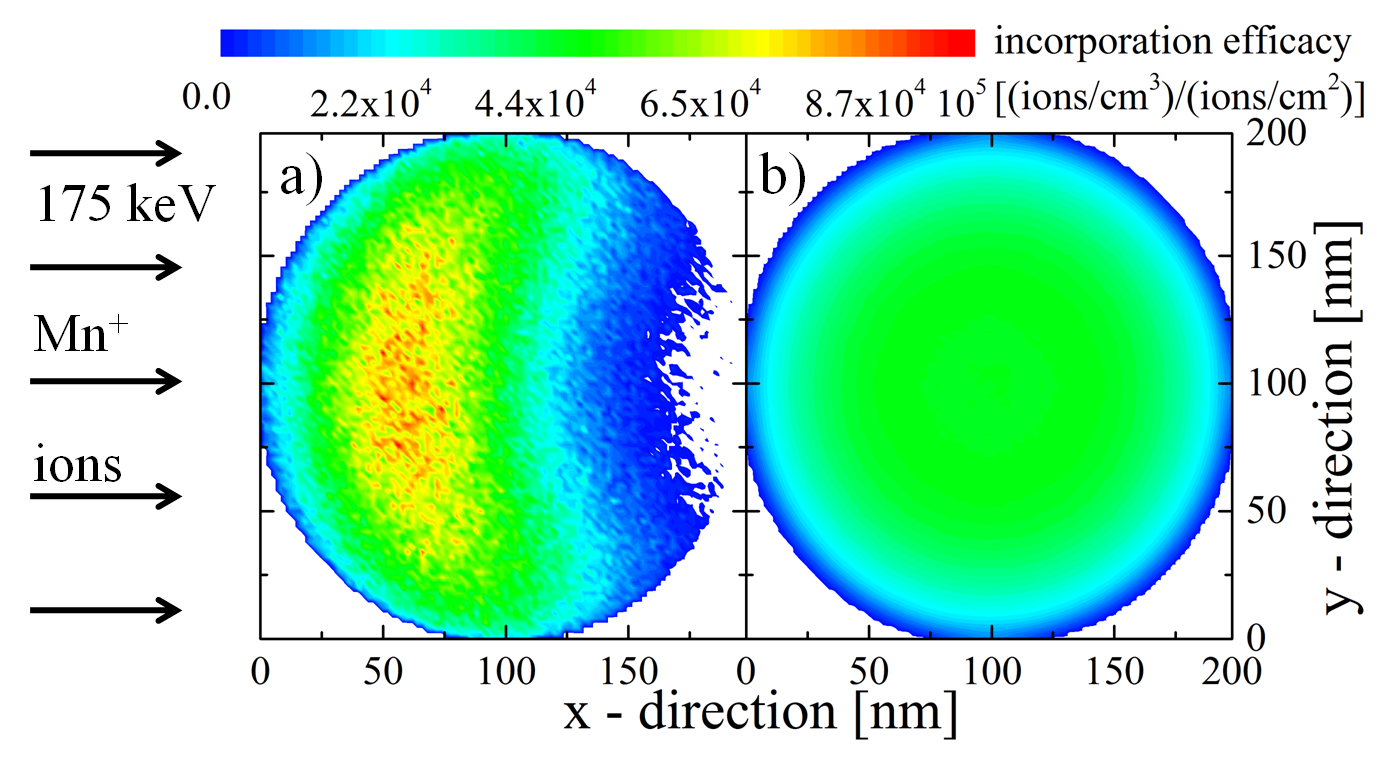
\includegraphics[width=.8\textwidth]{images/iradinacrosssection.png}
	\caption{a) Color plot of the concentration per ion fluence for the irradiation of a $200\,nm\,ZnO$ nanowire with $175\,keV\,Mn^+$ ions at an angle of $45^\circ$ to the $z$-axis. The energy was selected so that the rotation of this profile produces a radially homogeneous dopant distribution, as shown in b). The mean dopant incorporation efficacy is $3.6\cdot10^4\,\nicefrac{(atoms/cm^3)}{(ion/cm^2)}$ in both cases.}
	\label{iradinacrossection}
\end{Figure} 

Because lower energy ions have lower ranges, there are fewer paths that cause the ion to leave the nanowire, particularly in the forward direction. Therefore, the first advantage of decreasing the ion energy is that the doping efficacy is larger for lower ion energies, so a lower irradiation ion fluence is required to achieve doping at a desired concentration. Furthermore, lower ion energy impacts also produce less damage in the irradiated matrix. Together with an optimal irradiation temperature, the rotated irradiation was utilized to improve the magnetic properties of $Mn^+$ irradiated $GaAs$ nanowires in references \cite{borschel_new_2011,paschoal_hopping_2012,borschel_ion-solid_2012,kumar_magnetic_2013,paschoal_magnetoresistance_2014}. 


%In Figure \ref{iradinacrossection}b the outermost layer of the nanowire has a lower dopant incorporation efficacy than the rest of the wire volume. The sputtered atoms predominantly originate from this outer layer, so that the matrix of the nanowire is eroded preferentially to the incorporated dopants. 


\section{nano-XRF on single nanowires}

The increase in doping concentration with the irradiated ion fluence was investigated on $ZnO$ nanowire samples grown in Jena. The samples such as the one shown in Figure \ref{ZnOnanowires}a show an upstanding, dense forest of nanowires on the growth substrate. The nanowires were rotated during the irradiation with $0.24, 0.48, 0.95$ and $1.9\cdot 10^{17}\,\nicefrac{ions}{cm^2}\,Mn^+$ ions at $175\,keV$; corresponding to $Mn/Zn$ ratios of $0.02, 0.04, 0.08$ and $0.16$, as extrapolated from the mean doping efficacy obtained from the \emph{iradina} simulation. After the irradiation, they were transferred onto the $C$-foil of a $Cu$-TEM grid by imprinting.

\begin{Figure}[h]
	\centering
		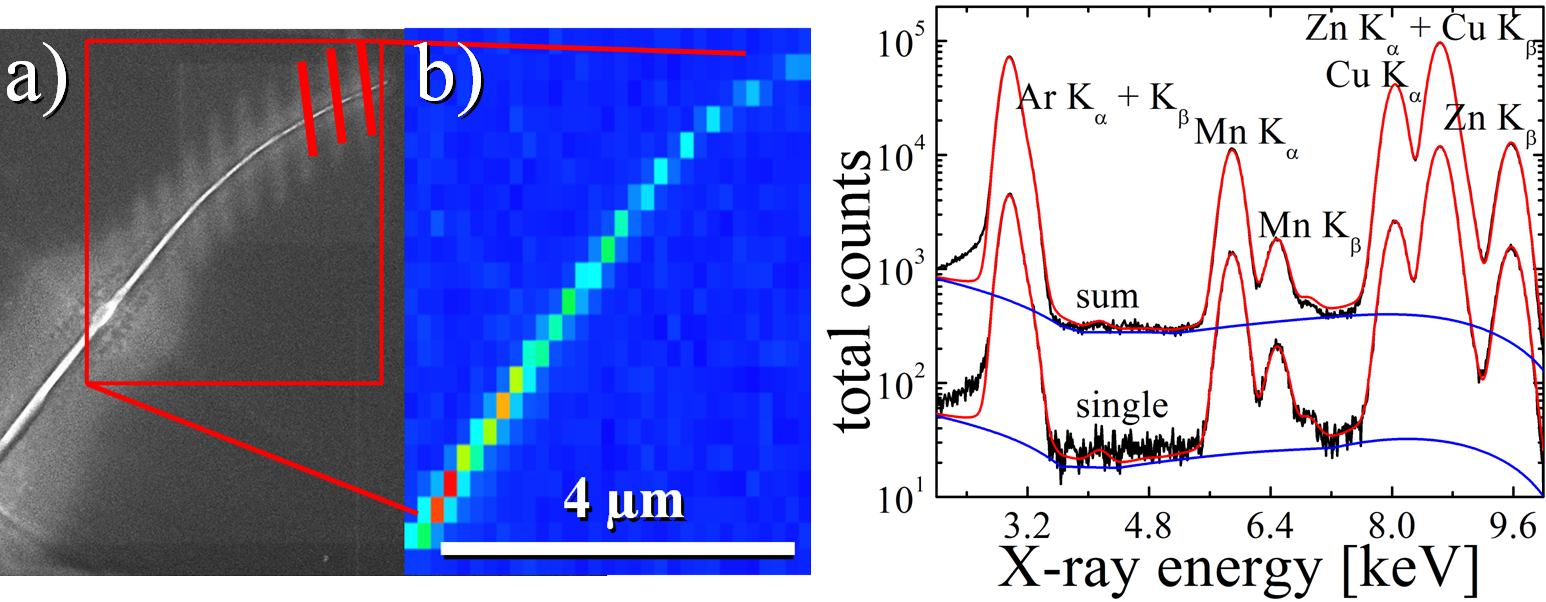
\includegraphics[width=.8\textwidth]{images/XRFSEM.png}
	\caption{a) SEM image of a $175\,keV\,Mn^+$ irradiated $ZnO$ nanowire on the carbon-foil of a $Cu$ TEM grid after XRF investigation. The red lines indicate where the focused X-ray beam was scanned with a long integration time. b) Intensity map of the X-ray signal from the nanowire shown in a). The black lines in c) show exemplary measured XRF-spectra of a single scanned line and for the sum of all the lines for the nanowire shown in a) and b). The fitted background and XRF-spectra are shown by blue and red lines.} 
	\label{XRFSEM}
\end{Figure} 


Figure \ref{XRFSEM}a shows a SEM image of one of the $Mn^+$ irradiated $ZnO$ nanowires after investigation by nano-XRF at the ESRF. The nanowire shows some damage a one point where the exposure to the XRF-beam was accidentally prolonged during the navigation on the sample. Also the track of the intense, focused X-ray beam can be seen on the carbon foil by some redeposition of material. All in all, the damage to the nanowire is, however, not large enough to have an effect on the quantification, especially considering that this particular nanowire was selected because it showed the most pronounced effects. In Figure \ref{XRFSEM}b a map of the detected X-ray intensity clearly shows the nanowire. The XRF spectrum collected for one of the scans indicated in the SEM image \ref{XRFSEM}a is shown in \ref{XRFSEM}c. The number of counts for a single scan is comfortably sufficient to quantify the $Mn$ and $Zn$ content. The average concentration for a nanowire was determined by fitting the sum XRF-spectrum of all scans across the nanowire.

In Figure \ref{MnZn1}a the $Mn/Zn$ ratio is plotted over the position along the nanowires' length for the four nominal concentrations. Clearly, there is a significant gradient in the $Mn$ concentration along the nanowire length. The maximum $Mn/Zn$ ratio was always found at the tip of the nanowires. The tip of the nanowires could be identified in the SEM images by the tapering of the nanowires. The $Mn/Zn$ ratio for both the sum of all scans, as well as the scan at the tip showing the maximum $Mn/Zn$ ratio, is plotted in \ref{MnZn1}b alongside the nominal ratio extrapolated from \emph{iradina} simulations.

\begin{Figure}
	\centering
		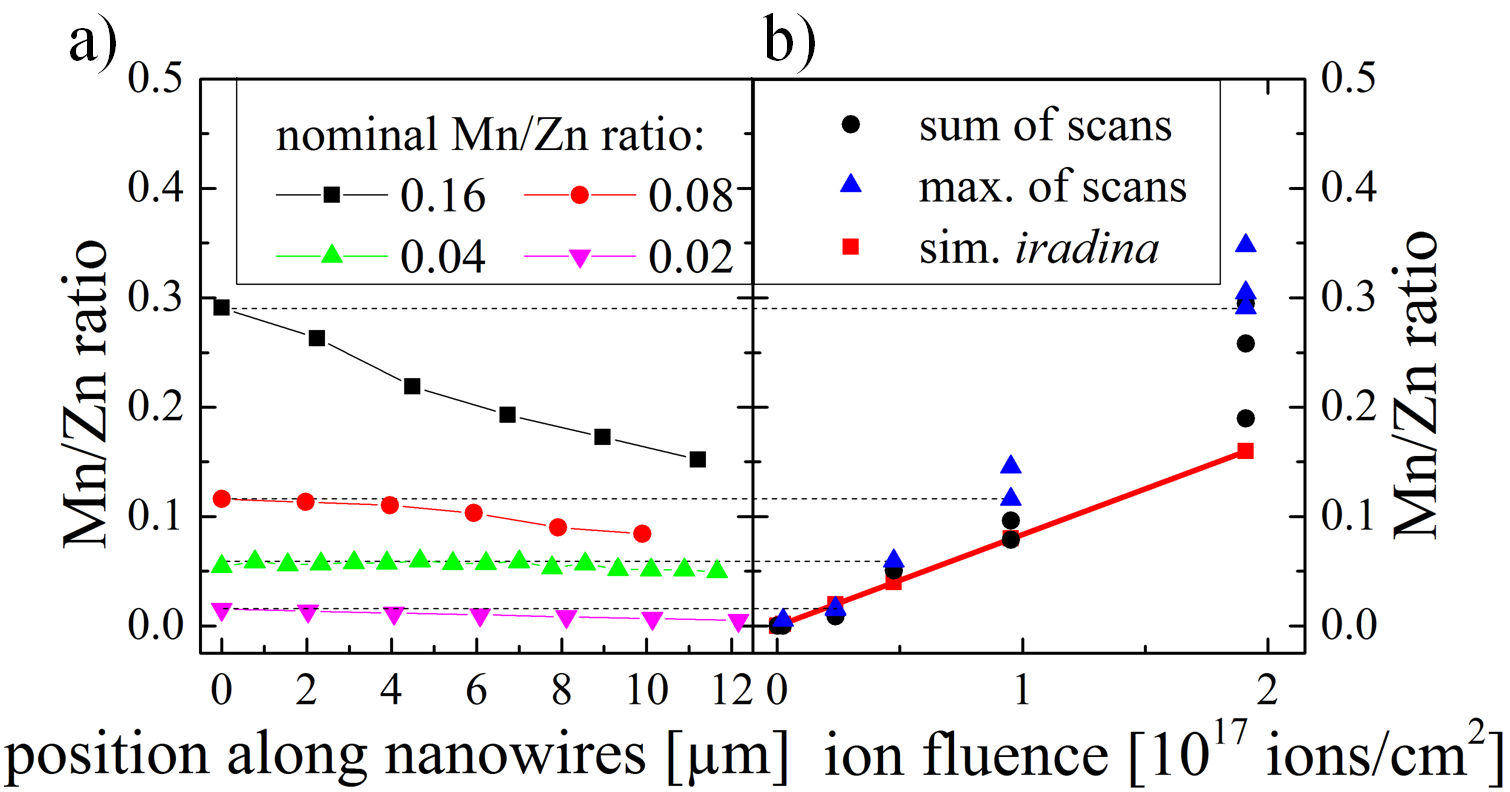
\includegraphics[width=.8\textwidth]{images/MnZn1.png}
	\caption{a) $Mn/Zn$ ratio quantified with PyMCA for representative wires along the length of the nanowires for varying nominal concentrations. The tip of the nanowires is found at $0\,\mu m$. In b) the black circles show the average ratio obtained for various nanowires by fitting to the sum of all scans. The blue upturned triangles show the maximum ratio found along the length of the nanowires. The corresponding data points in the plot of the concentration versus the length of the nanowire in a) are connected with a dashed line. The red data points and line in b) indicate the linear extrapolation to the nominal $Mn/Zn$ ratio from \emph{iradina} simulations.}
	\label{MnZn1}
\end{Figure} 
 
Two pieces of information can be gained from these results. First, the nanowires on the sample clearly shadowed each other from the ion beam, leading to the pronounced $Mn$ concentration gradient along the wires' length. The shadowing is least at the tips of the nanowires, therefore these points correspond closest to the simulated situation. The shadowing also causes a tapering of the nanowires towards the tip, because the material sputtered away increases with increasing exposure to the ion beam. The second point is that the increase in $Mn$ concentration per ion fluence is much stronger than the linear extrapolation from static simulations. Using the doping efficacy gained from the earlier simulations to calculate the required ion fluence for a desired doping concentration assumes, that the concentration increases linearly with the irradiated ion fluence. However, this is only true in the absence of sputtering. Sputtering erodes the target nanowire at the same time as ions are incorporated. It thus leads to a non-linear increase in the concentration of dopants with the irradiated ion fluence. To separate the effect of shadowing amongst the nanowires from the sputtering of each individual nanowire, the irradiation and quantification has to be repeated with nanowires with a sparser lateral distribution, as shown in Figure \ref{ZnOnanowires}b. These were kindly provided by Dr. Helena Franke from the University Leipzig.


\begin{Figure}[th]
	\centering
		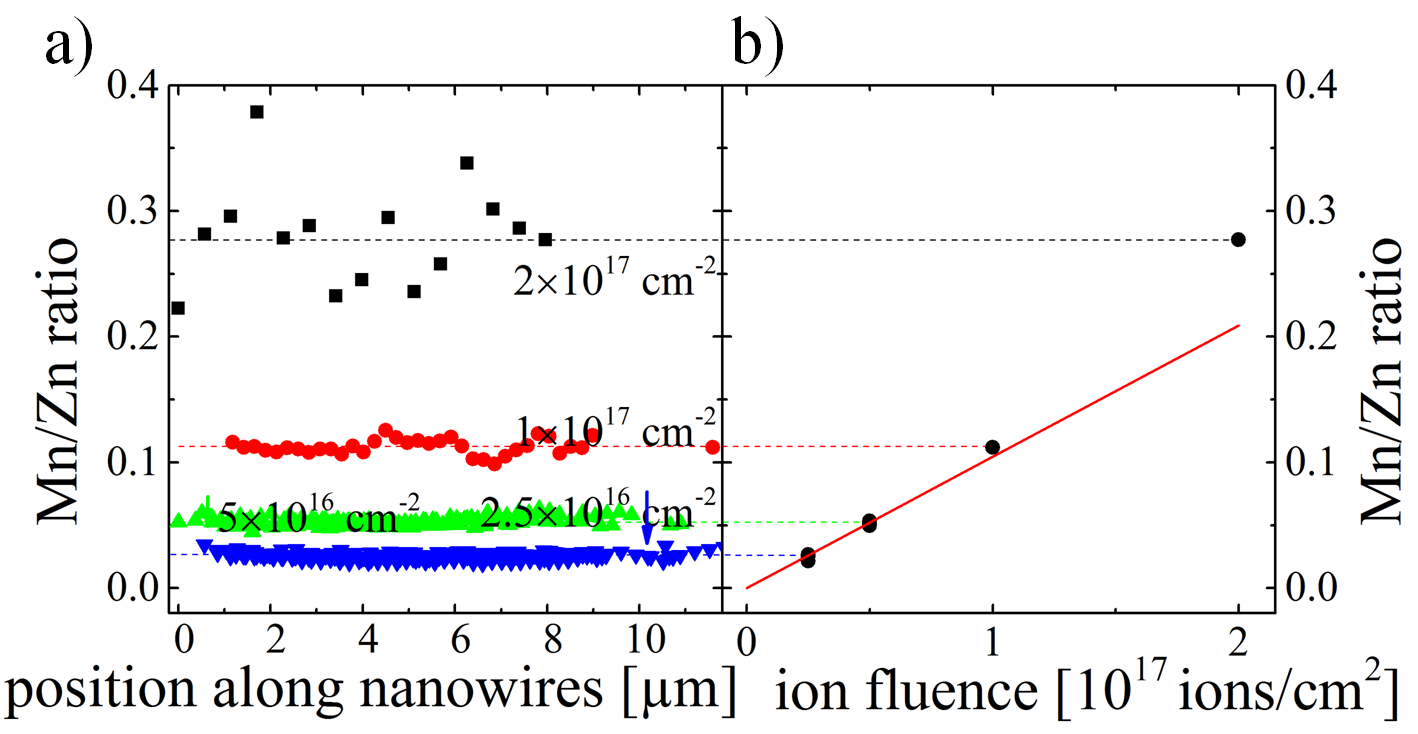
\includegraphics[width=.85\textwidth]{images/MnZn2.png}
	\caption{a) $Mn/Zn$ ratio along the wire length for sparse nanowire samples irradiated with the indicated ion fluence of $175\,keV Mn^+$. There is no concentration profile along the wire length. In b) the average ratio obtained by fitting to the sum of all scans for the respective ion fluence is shown. The red line in b) shows the linear extrapolation from \emph{iradina} simulations.}
	\label{MnZn2}
\end{Figure} 

The same nano-XRF quantification procedure was followed to investigate the $Mn/Zn$ ratio after the irradiation of these sparser nanowire samples with $0.25, 0.5, 1$ and $2\cdot 10^{17}\,\nicefrac{ions}{cm^2}$ of $175\,keV\,Mn^+$. The results are shown in Figure \ref{MnZn2}. The $Mn/Zn$ ratios plotted against the nanowire length in \ref{MnZn2}a no longer show any gradient. The $Mn/Zn$ ratio for the nanowires irradiated with higher ion fluences shows a significant spread because the thinned nanowires have a much smaller volume and thus give a lower total XRF signal. Added to this, the thinner wires could only be attached to the lacy carbon loosely, so that they drifted much more during the XRF scans making it impossible to increase the integration time significantly to compensate for the lower signal. 

\begin{SCfigure}[50][h]
	\centering
		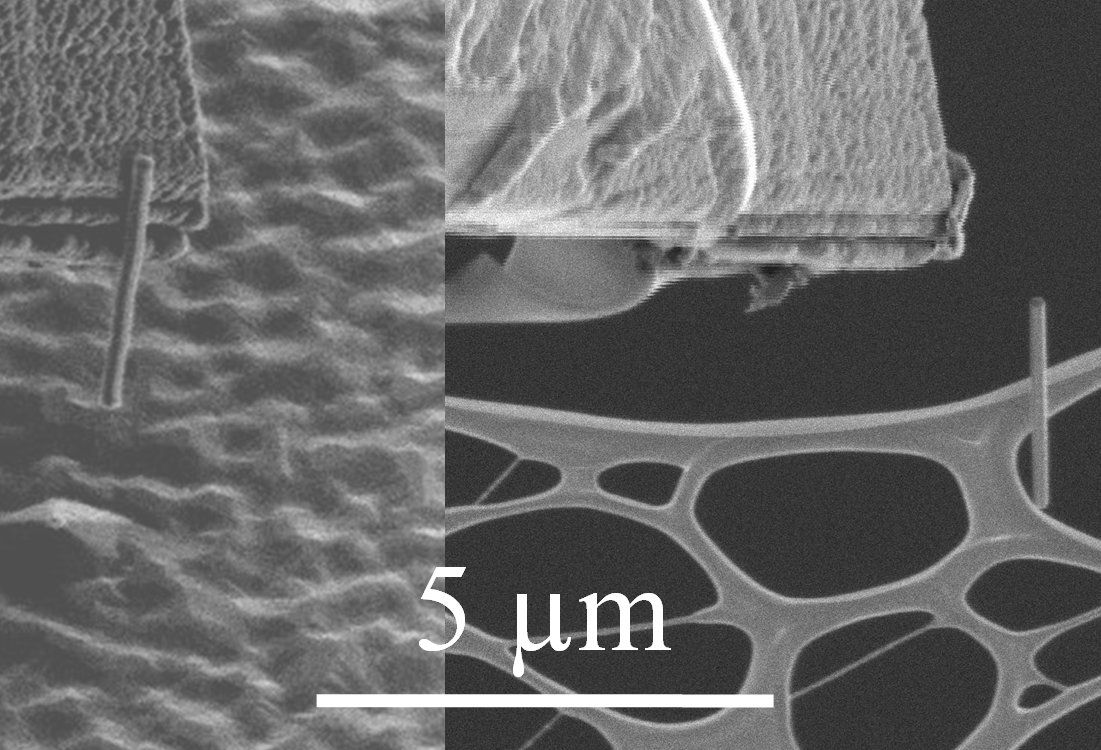
\includegraphics[width=.5\textwidth]{images/SEMbreak.png}
	\caption{SEM images showing a ZnO nanowire broken off the growth substrate (left) with a micro-manipulator and transferred onto the lacy carbon-foil on a commercial TEM grid (right). Using this technique, individual nanowires investigated by SEM before and after the irradiation could be selected for subsequent nano-XRF quantification.}
	\label{SEMbreak}
\end{SCfigure}

As shown in Figure \ref{SEMbreak}, these wires were individually transferred to the lacy carbon TEM grid so that nanowires, which were investigated by SEM before and after irradiation, could be selected. For example, the diameter of the nanowire irradiated with the highest ion fluence was reduced from $202\,nm$ to $93\,nm$ by sputtering. The nanowires irradiated with lower ion fluences showed lower reductions in their diameters, as expected. From these diameter reductions the sputter yield can be calculated, resulting in sputter yields in the range of 5 - 20$\,\nicefrac{atoms}{ion}$. As seen in the dedicated study of sputtering in Chapter \ref{sec:sisputtering}, these values have a very large spread. 

The determined average $Mn/Zn$ ratio is plotted in \ref{MnZn2}b against the irradiated ion fluence for all irradiated fluences. It is accurate to within $\pm\,0.01$, because it is based on the sum of the spectra of all the individual scans. This sum-spectrum includes a sufficiently large number of counts in all instances. The initial increase in the $Mn/Zn$ ratio with the irradiated ion fluence closely follows the linear extrapolation from the doping efficacy for fluences up to $0.5\cdot 10^{17}\,\nicefrac{ions}{cm^2}$. This is an important result, because it confirms that the MC BCA simulation can accurately predict the incorporation of dopants quantitatively. Therefore, the doping efficacy is a useful number to determine the required ion fluence for a desired doping concentration for low ion fluences, were sputtering is not yet significant. However, as with the denser nanowire sample, for high ion fluences the increase in the $Mn$ concentration is much larger than the simple linear extrapolation from the \emph{iradina} simulation. The fact that there is no longer a gradient in the concentration along the nanowire length for the sparser samples confirms that the previously observed, strong gradient in the incorporation was caused by the shadowing of the nanowires amongst themselves.


\section{Pseudo-dynamic simulation}

The direct simulation of the effect of sputtering on the incorporation of dopants into nanowires requires a dynamic simulation program which also considers the three dimensional geometry of the target. Because such software is currently not openly available, a step-by-step investigation using results from static simulations will be undertaken to discuss the observed interaction between dopant incorporation and sputtering.

\begin{SCfigure}[][h]
	\centering
		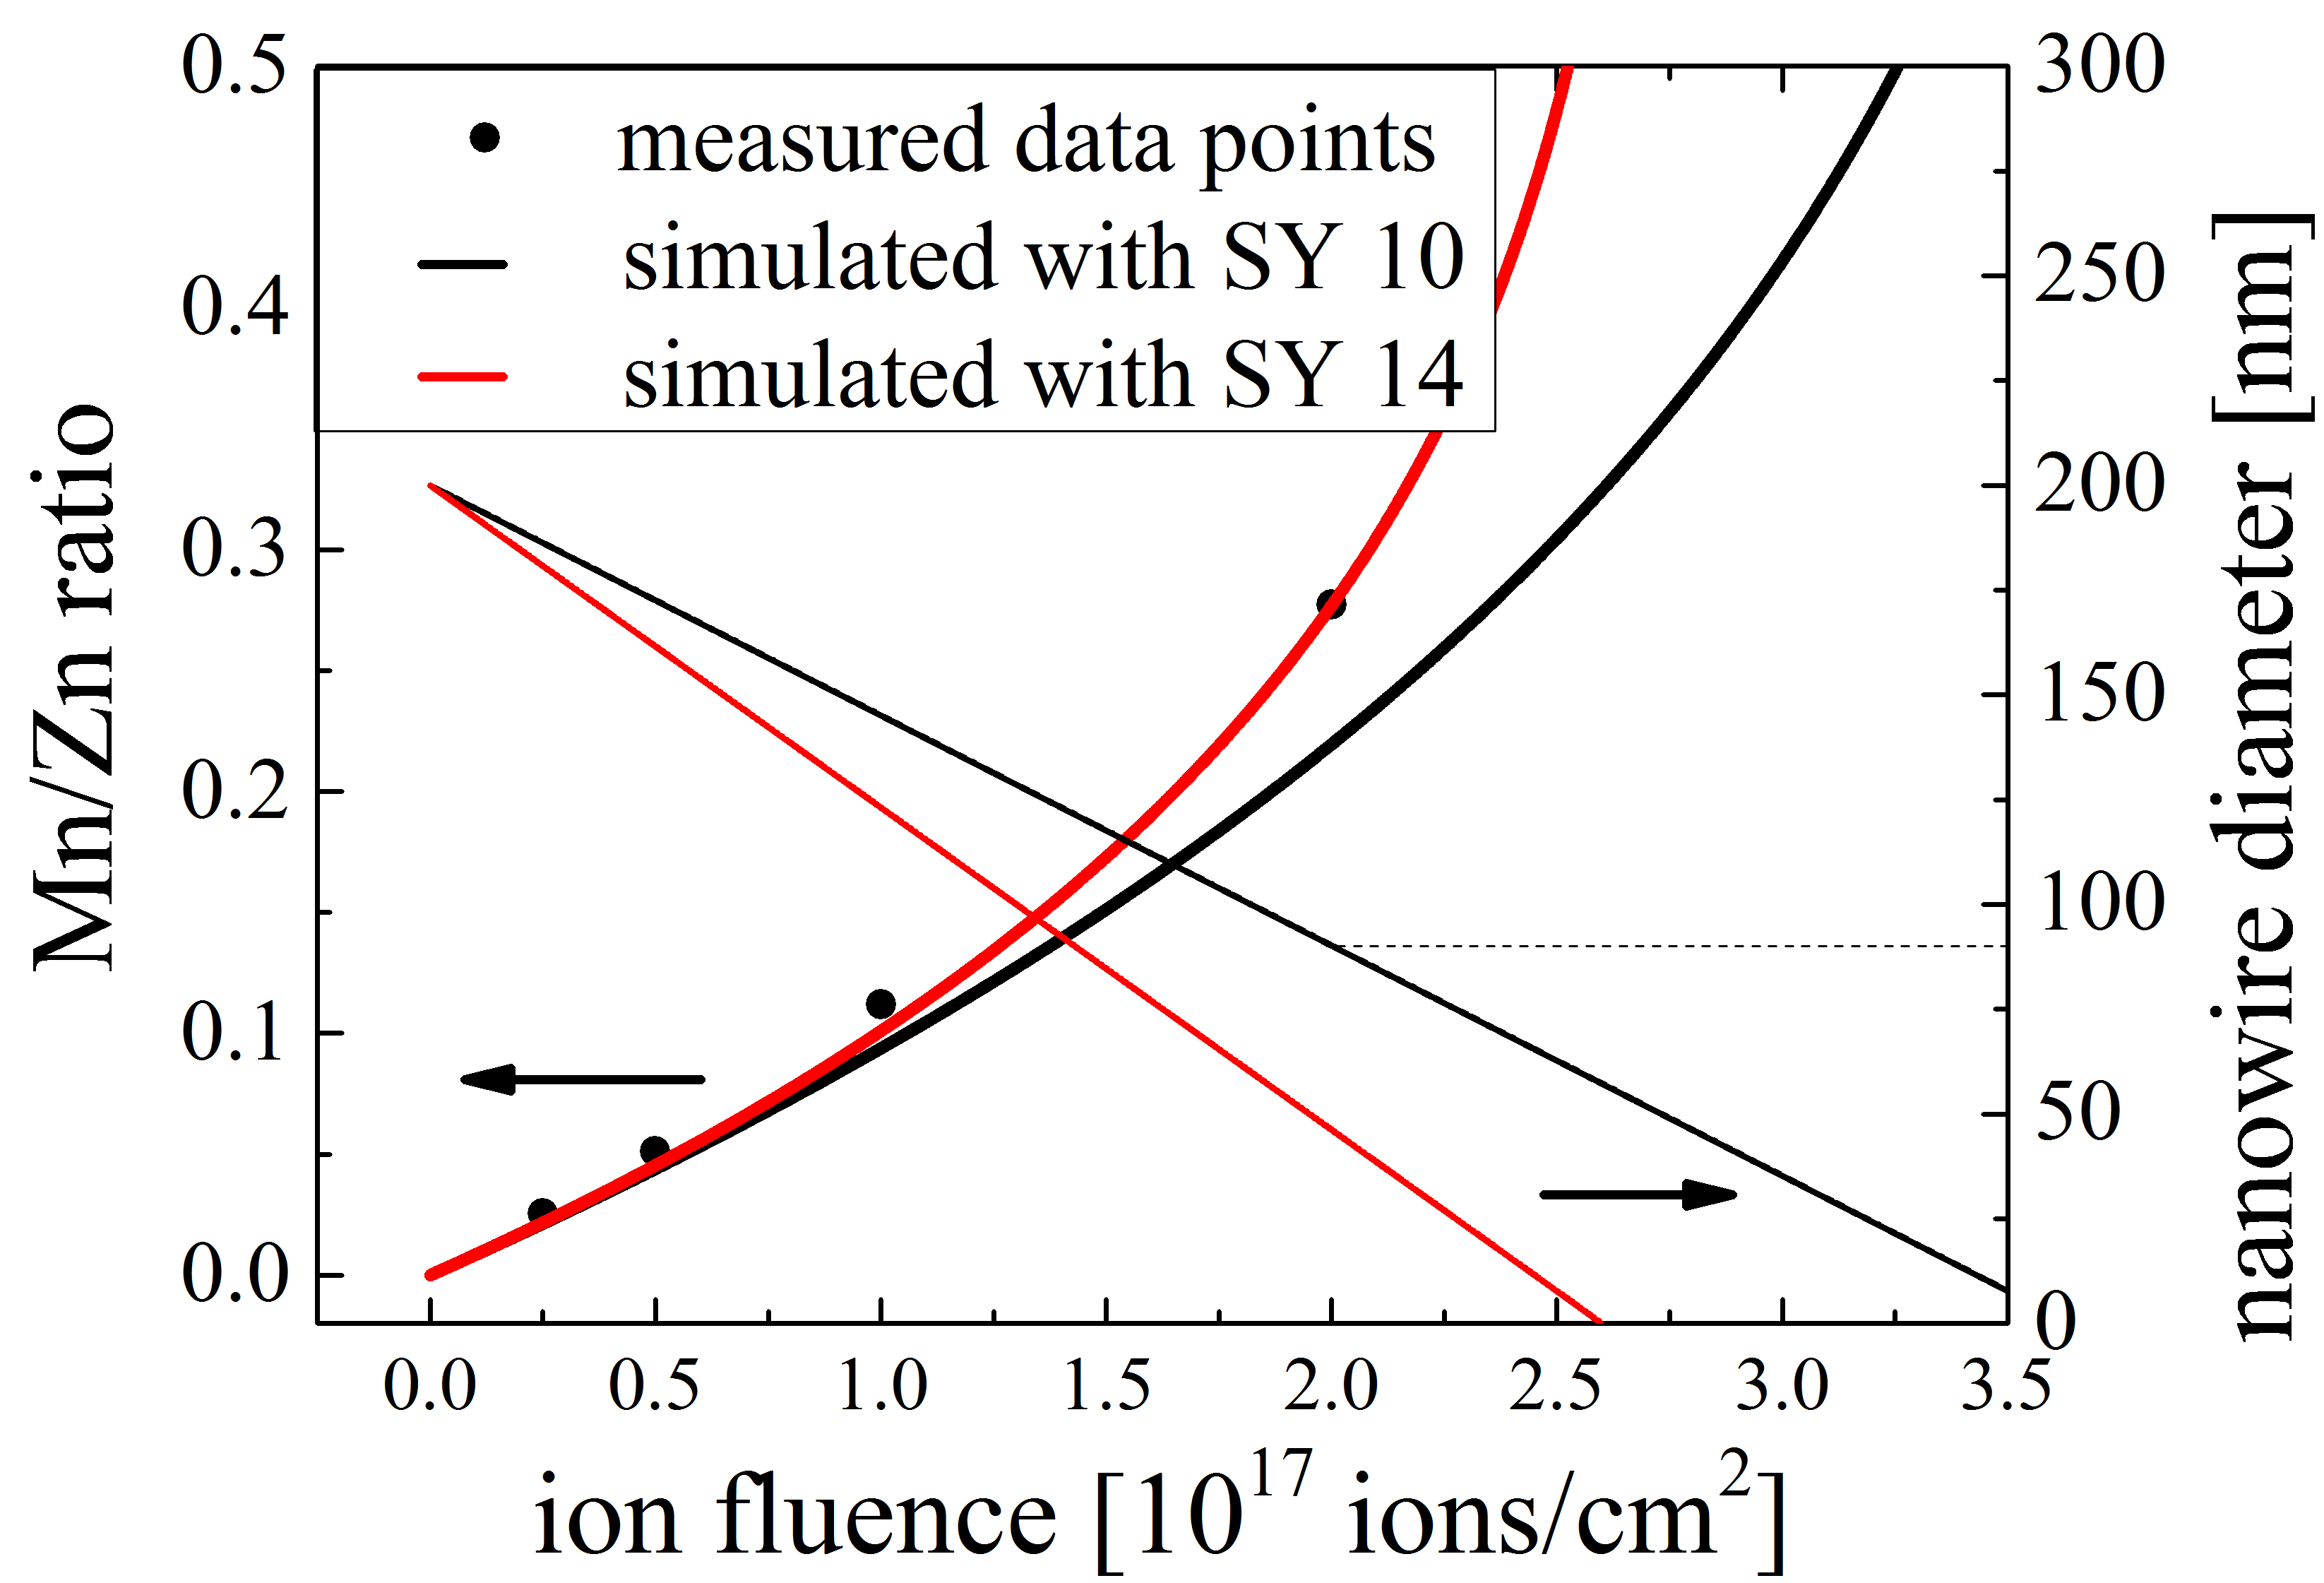
\includegraphics[width=.5\textwidth]{images/staticsputteryield.png}
	\caption{Plot of the $Mn/Zn$ ratio (left axis) versus the irradiated ion fluence of $175\,keV Mn^+$ for the measured nanowires and two simulations using different sputter yields. The nanowire diameter (right axis) is also plotted against the ion fluence for both simulations. The dashed line at $90\,nm$ marks the final radius of the data point corresponding to the highest irradiated fluence.}
	\label{staticsputter}
\end{SCfigure} 

The most straightforward approach is to consider the total sputter yield and the doping efficacy to be constant. With these assumptions and a reiterative calculation of incremental ion fluence steps, a pseudo-dynamic simulation can be numerically constructed. The $Mn$ concentration increases with each irradiated incremental ion fluence step by the value determined by the doping efficacy. Then the number of $Zn, O$ and $Mn$ atoms is reduced by sputtering in such a way, that the total sputter yield is divided between $Zn+O$ and $Mn$ according to the current $Mn$ concentration. The total number of atoms is used to calculate the new nanowire radius and the next incremental ion fluence step can be calculated.

Figure \ref{staticsputter} shows the experimentally determined $Mn/Zn$ ratios next to such a simulation. The doping efficacy was set to the same value used for the linear extrapolation: $3.6\cdot10^4\,\nicefrac{(atoms/cm^3)}{(ion/cm^2)}$. The total sputter yield was set to $10\,\nicefrac{atoms}{ion}$ for the simulation yielding the values depicted in black. This sputter yield value corresponds to the sputter yield determined from the reduction in the radius of the nanowire irradiated with $2\cdot10^{17}\,\nicefrac{ions}{cm^2}$ and therefore, unsurprisingly, this simulation produces the the correct diameter of $\approx\,90\,nm$ at this ion fluence. However, the calculated $Mn/Zn$ ratio is too low. Conversely, a simulation with a larger sputter yield of $14\,\nicefrac{atoms}{ion}$, indicated in red, correctly reproduces the $Mn/Zn$ ratio, but erodes the nanowire too quickly. Nevertheless, the overall agreement between the experiment and the simulation seems promising and confirms that the super linear increase in the doping concentration observed in the experiment can be explained by the sputtering of the nanowire.

\begin{Figure}
	\centering
		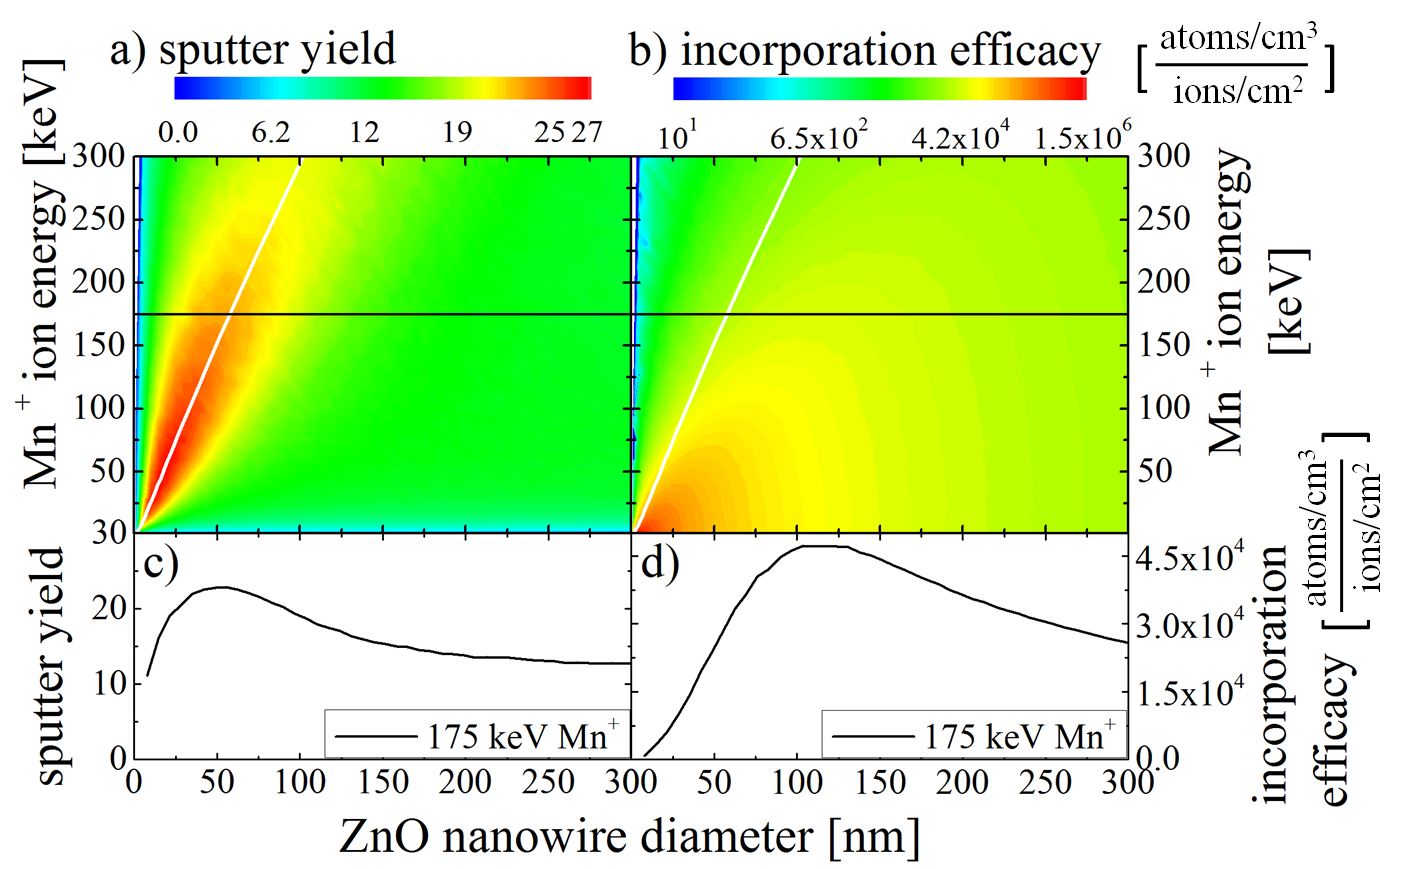
\includegraphics[width=.8\textwidth]{images/sputterincorporate.png}
	\caption{a) Sputter yield for the irradiation with $Mn^+$ of ZnO nanowires with varying diameters an ion energies. From the same simulations the dopant incorporation efficacy was determined and plotted in b). The white line in both plots indicates the ion range at the respective energy and $45^\circ$, calculated with SRIM for $Mn^+$ in $ZnO$. The horizontal black line indicates the ion energy used in the experiments and simulations in this Chapter. For this energy the diameter-dependent sputter yield and doping efficacy are plotted in c) and d) respectively.}
	\label{sputterincorporate}
\end{Figure} 

To increase the accuracy of the pseudo-dynamic simulation, results from a set of static simulations for varying diameters can be used. The sputter yield is dependent on the nanowire radius and the ion energy as shown in figures \ref{sputterincorporate}a and \ref{sputterincorporate}c. This relation is discussed in detail in the previous Chapter \ref{sec:simsputering}. Likewise, the incorporation efficacy plotted in \ref{sputterincorporate}b is also dependent on the nanowire radius and the ion energy. For a fixed diameter and increasing ion energy the efficacy is monotonically decreasing, because the probability of the ion to leave the nanostructure rises together with the ion range. For a fixed ion energy, as shown in Figure \ref{sputterincorporate}d, the probability of an ion to stay in the nanostructure increases with increasing nanowire diameter, so that for small diameters the efficacy also increases with increasing diameter. For large diameters this effect is overcompensated by a stronger dilution of the dopants in the volume of the nanowire which increases as the square of the diameter. This leads to a maximum in the incorporation efficacy at diameters around twice the ion range. Note that the color scale in \ref{sputterincorporate}b is logarithmic, while the graph \ref{sputterincorporate}d has a linear scale.



The numerical, pseudo-dynamic simulation can easily be adapted to use the diameter-dependent values for the sputter yield and the dopant incorporation efficacy of figures \ref{sputterincorporate}c and \ref{sputterincorporate}d. As with the previous pseudo-dynamic simulation, which only considered constant sputtering and dopant incorporation efficacy, it is only possible to reproduce the correct diameter \underline{or} the $Mn/Zn$ ratio. For the results shown in Figure \ref{pseudodynamic} the diameter-dependent sputter yield used for the simulation had to be halved. A simulation with the full sputter yield shown in figures \ref{sputterincorporate}c already eroded the $200\,nm$ nanowire completely after the irradiation with an ion fluence of $\approx 1.5\cdot 10^{17}\,\nicefrac{ions}{cm^2}$. This is not a cause for concern, however, because the quantitative values for the sputter yield obtained by \emph{iradina} simulations are not expected to be reliable and the effective sputter yield will be reduced in a material which can (re)-oxidize. Both these points were already discussed in Chapter \ref{sec:sputter}.

\begin{SCfigure}[50][h]
	\centering
		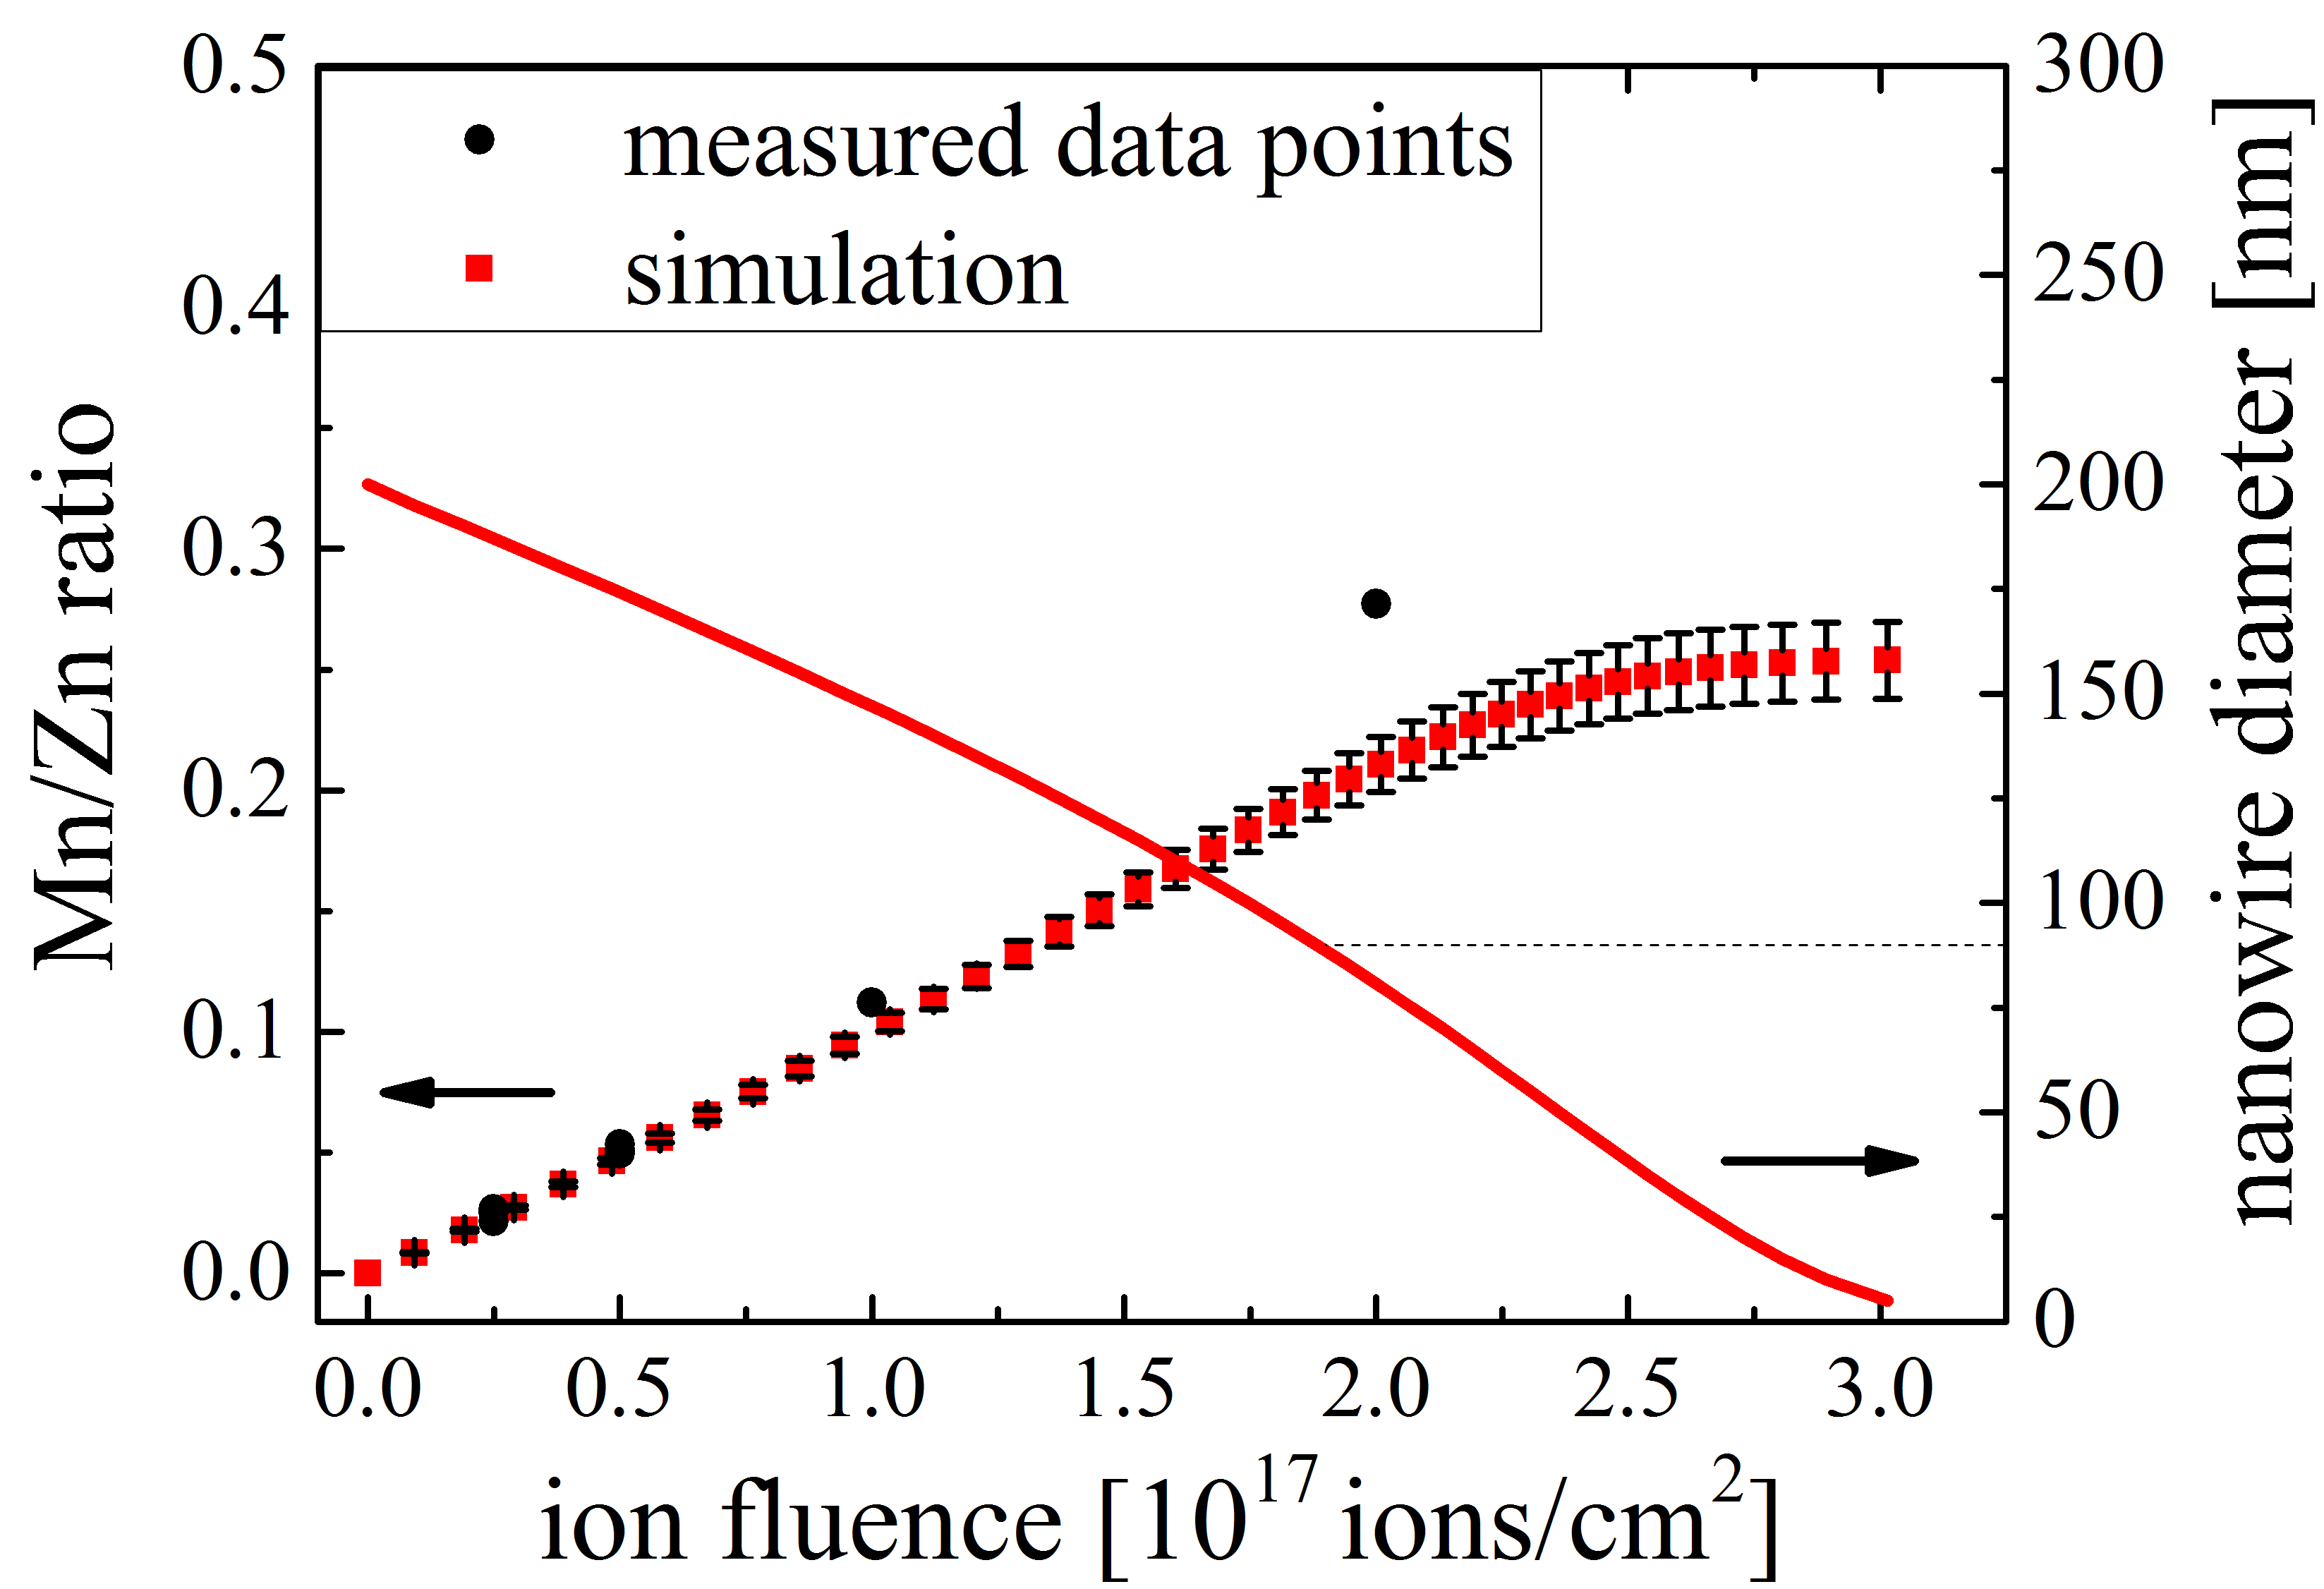
\includegraphics[width=.5\textwidth]{images/pseudodynamic.png}
	\caption{Results from a pseudo-dynamic simulation considering diameter-dependent sputtering and doping efficacy. The $Mn/Zn$ ratio is plotted to the left axis versus the ion fluence of $175\,keV Mn^+$ as red squares for the simulation and black circles for the experiment. The error bars range from the $Mn/Zn$ ratio for $170\,keV$ to $180\,keV Mn^+$. The red line indicates the simulated nanowire diameter.}
	\label{pseudodynamic}
\end{SCfigure} 

The resulting $Mn/Zn$ ratios from such a simulation are plotted in Figure \ref{pseudodynamic} as red squares. The stronger than linear increase in the $Mn/Zn$ ratio with the irradiated ion fluence is offset by the doping efficacy decreasing markedly with increasing ion fluence from $\approx 1.5\cdot 10^{17}\,\nicefrac{ions}{cm^2}$. Here, the nanowire has a remaining diameter of around $120\,nm$. At this diameter, the $175\,keV Mn^+$ ions start to reach the back of the now thinned nanowire, the sputtering increases and the doping efficacy decreases, as shown in figures \ref{sputterincorporate}c and \ref{sputterincorporate}d. In the evolution of the diameter with the irradiated ion fluence, plotted in Figure \ref{pseudodynamic} as a red line, the increased sputter yield is noticeable as a slight increase in the slope of the curve at $2\cdot 10^{17}\,\nicefrac{ions}{cm^2}$. 

Largely because of the reduced $Mn$ incorporation in thinned nanowires, the simulation fails to reproduce the measured $Mn/Zn$ ratio for ion fluences of $1\cdot 10^{17}\,\nicefrac{ions}{cm^2}$ and above, underestimating the $Mn$ concentration significantly. This is due to the assumption that the probability of sputtering a $Mn$ or a $Zn/O$ atom is determined by the average $Mn$ concentration in the nanowire. This would only be true if the doping profile were truly homogeneous. In reality there is a $Mn$ poor surface region in the doping profile shown in Figure \ref{iradinacrossection}b. In addition, as the nanowire is thinned during the irradiation, the homogeneity of the doping profile will also suffer. A peak emerges in the middle of the nanowire as the radius becomes equal to the ion range and smaller. In summary, this means that more $Zn$ and $O$ atoms are sputtered from the nanowire than predicted by the $Mn$ concentration weighted sputter yield and that the core is enriched in $Mn$ faster than the averaged doping incorporation efficacy would suggest. When the outer $Mn$ poor layers of the nanowire are sputtered away, the $Mn/Zn$ ratio averaged over the whole cross-section increases, even without the additional incorporation of $Mn$. At this point it no longer makes sense to try to predict doping concentrations with static simulations, which cannot take into account the change in the target composition and geometry. Dynamic simulations are required.
 

\section{Summarizing Discussion}

The incorporation of dopants into nanowires was studied by investigating $Mn$ irradiated $ZnO$ nanowires with nano-XRF. The first, perhaps slightly obvious result is that the doping concentration can be significantly influenced by shadowing of the nanowires amongst themselves. This sets some limits on the suitability of samples for homogeneous irradiation. The dense and disordered samples investigated in previous work on ion irradiated nanowires \cite{geburt_rare_2008,ronning_ion_2010,kaiser_defect_2011,geburt_lasing_2012,geburt_intense_2013,kaiser_luminescence_2013,geburt_intense_2014,chu_nano-x-ray_2014} for example, are very likely to show a large spread in the locally realized doping concentration. Related to this fact is the insight that control of the irradiation geometry can greatly reduce both the energy and ion fluence required to obtain a homogeneous doping concentration. The possibility of irradiation from different angles was realized in the presented case by rotation of the target. Both a reduced energy and a reduced ion fluence reduce the total damage produced in the target and can elevate the annealing requirements and thus improve the properties of doped nanowires \cite{borschel_new_2011,paschoal_hopping_2012,borschel_ion-solid_2012,kumar_magnetic_2013,paschoal_magnetoresistance_2014}. In any case, it was already shown that irradiated nanowires can bend in either direction relative to the ion beam, depending on the ion energy \cite{borschel_permanent_2011}. The rotated irradiation is a practicable alternative to complex modulations of the ion energy, which could also prevent unwanted bending of nanowires during the irradiation with high ion fluences.

The quantification of the dopants in irradiated nanowires showed that the static MC BCA code \emph{iradina} is accurate in the prediction the doping concentration for low ion fluences. This was expected from the discussion in Chapter \ref{sec:simion} on the underlying scientific background for the direct simulation of ion trajectories which translates well into nanostructures and thus naturally gives an accurate prediction of the final distribution of the ions in the target. However, because of sputtering, a reasonable upper limit to the applicability of static simulations seems to be given in these experiments by an ion fluence of $0.5\cdot 10^{17}\,\nicefrac{ions}{cm^2}$. This corresponds to the reduction of the nanowires diameter by about $10\%$, or a reduction of the nanowire volume by roughly $20\%$. Note, that this result can be generalized to other target materials, ion species and ion energies only if the ion range is comparable or larger than the nanowire diameter. For low ion energy irradiation, where the ion range is also low, the sputtering will effect the doped volume of the nanowire much sooner! The same holds true for other nanostructured geometries. A dynamic simulation is required once the sputtered layers amount to a sizable portion of either the implanted ion range or of the characteristic nanostructure length, which ever is smaller. 

For flat target geometries, dynamic simulation tools have been available for some time \cite{moller_tridyn_1984,moller_tridyn-binary_1988} and comparisons between simulations and experiments in studies on high fluence irradiation in thin layers and bulk targets have already observed the influence of sputtering on the doping concentration \cite{miyagawa_computer_1991,sigmund_alloy_1993}. Unlike in nanowires, the material loss through sputtering is insignificant to the total bulk volume. However, as with the irradiation of nanostructures with low ion energies, the sputtered depth has to be compared with the ion range. When both become comparable, the interplay between sputtering and incorporation depth of dopants can lead to strong dynamics, including an oscillation of the dopant concentration along the depth of the target \cite{eckstein_oscillations_2000}. 

Unfortunately, there is no straightforward way to extend the usefulness of static simulations to higher ion fluences. Although the attempted pseudo-dynamic simulations were partly able to reproduce the incorporated doping concentration or the nanowire radius, this was only possible in retrospect and by altering the simulation parameters. A predictive algorithm that is not dynamic was not found. The problem caused by the inhomogeneous incorporation of the dopant and the disproportionately large sputtering of the nanowire material can only be solved by dynamic codes, which consider both the nanostructure geometry, as well as the local concentration of each element in the target geometry. Such simulation tools are under development, if not openly available yet \cite{moller_tri3dyn_2014}.

Even in dynamic simulations, a remaining problem is posed by the sputter yield, which is not easy to simulate correctly. The case for single element materials was discussed in Chapter \ref{sec:sputter} on sputtering, but in compound or highly doped materials, the problem is significantly complicated by the possibility of preferential sputtering of specific elements. In flat geometries, both the preferential sputtering of the incorporated dopant, as well as compositional changes in compounds and alloys can drastically change the final composition of the irradiated layer \cite{kelly_attempt_1978,moller_tridyn_1984,andersen_computer_1986,moller_tridyn-binary_1988,sigmund_alloy_1993,zaporozchenko_preferential_1995}. Due to preferential sputtering, an irradiated nanowire of a compound material may already be deficient in one of its components before a high dopant concentration is reached. At least in bulk samples the evolution of the concentration profiles for high fluence irradiations have a steady state solution. Because of mass conservation, the composition of the sputtered material is ultimately equal to the bulk material composition, which lies underneath an unstoichiometric layer effected by the irradiation \cite{andersen_computer_1986}. Nanowires and other nanostructures, on the other hand, are destroyed by sputtering and steady state conditions cannot arise for high fluences. The evolution of their composition for high ion fluence irradiation is therefore much less predictable.
